\documentclass[11pt,onecolumn]{witseiepaper}
\usepackage{KJN}
\usepackage{graphicx}

\usepackage[final]{pdfpages}
\usepackage{placeins}
\usepackage{siunitx}
\usepackage{amsmath}
\usepackage{caption}
\usepackage{subcaption}
\usepackage{tcolorbox}
\usepackage{adjustbox}
\usepackage{pgfplotstable}
\usepackage{pgfplots}
\usepackage{multirow}
\usepackage{graphicx}
\usepackage{placeins}
\usepackage{longtable}
\usepackage{color, hyperref} 
\usepackage{float}
\usepackage{tikz}
\usepackage{placeins}
\usepackage{listings}
\usepackage[framemethod=TikZ]{mdframed}
\definecolor{blue(ryb)}{rgb}{0.19, 0.286, 0.6}
\usepackage{breakurl}
\usepackage{tikzpagenodes}
\usepackage{pifont}% http://ctan.org/pkg/pifont
\newcommand{\cmark}{\ding{51}}%
\newcommand\tab[1][1cm]{\hspace*{#1}}
\usepackage[style=ieee, sorting=none]{biblatex}
\addbibresource{ref.bib}
\pagestyle{plain}
\begin{document}

\begin{titlepage}
\begin{center}
 

%
\includegraphics[width=0.4\textwidth]{EIE_Logo_Full_Colour.pdf}
 
\begin{minipage}{0.30\linewidth}
\centering

\includegraphics[height=8\baselineskip]{EIE_better.pdf}
\end{minipage}
\begin{minipage}{0.6\linewidth}
\centering
{\Large School of Electrical \& Information Engineering} \\
{\large University of the Witwatersrand, Johannesburg \\
Private Bag 3, 2050, South Africa}
\end{minipage}

\vspace{0.5cm}
\centering
\begin{tcolorbox}[width=\linewidth, colframe=blue(ryb), colback=blue(ryb), sharp corners=east,sharp corners= west]
\centering
{\color{white} {\large ELEN4011 - Design Project}\\
Biomedical Engineering - Design of an Adaptive Hearing Aid\\
23 October 2018}
\end{tcolorbox}

\vspace{3cm}

{\bf Supervisor:} Prof. D. Rubin 

\vspace{3cm}

\textit{Daniel Edwards\\
1055301}


\end{center}
\end{titlepage}

\tableofcontents
\newpage

\section*{Abstract}

This is my abstract

\section{Introduction}

define what adaptive means

\section{Background}

\noindent Hearing loss is a common problem in society. In \textit{2016}, the University of the Witwatersrand released a statement saying that in South Africa, approximately $20\%$ of the population suffers from a form of hearing loss \cite{witsHearingStats}. As a result of hearing loss, an individual can suffer from loneliness, isolation, dependence, depression and frustration. These are signs of poor quality of \cite{qualityOfLife}. The amount of people with an impaired quality of life provides motivation for the necessity of devices to improve an individuals hearing namely; a hearing aid to improve the patients speech intelligibility. 


\section{Design Research}

\noindent Many factors contribute to hearing loss. A common type is conductive hearing loss \cite{earinfo}. This is a result of age, excessive noise or various diseases \cite{hearIt}. This is a permanent form of hearing loss which can be treated with hearing assisting devices \cite{hearIt}. This section presents an analysis of existing solutions to this problem (Section \ref{sec:existSoln}) and a literature review (Section \ref{sec:litReview}).

\subsection{Existing Solutions}
\label{sec:existSoln}

make it for conductive here

\noindent Two main hearing assisting devices exist for sensorineural hearing impairments namely; hearing aids and cochlear implants \cite{atlantic}. Cochlear implants are typically used in cases of extreme hearing loss. These devices work well in quiet environments \cite{carroll}. However, cochlear implant users battle to perceive speech in noisy environments \cite{carroll} and thus, the individuals quality of life is not improved. Therefore, this design will make use of hearing aid technology.\\
\newline
\noindent There are two main types of hearing aids, analog and digital. Analog hearing aids amplify all sounds, including noise\cite{woodford}. Ricketts \cite{ricketts} states that the largest problem for the hearing impaired is listening in noisy situations. Digital hearing aids however, contain a signal processing element which gives them additional functionality such as filtering noise, and isolating sounds in specific directions \cite{ricketts}. Thus, these hearing aids improve the patient's speech intelligibility which can positively their social experience.\\

put something in about Ricketts and avoiding noise - isolation, say something about adaptive

\subsection{Literature Review}
\label{sec:litReview}

\noindent Sebastian \textit{et al.} \cite{sebastian} define a hearing aid, as an electro-acoustic device with the purpose of making speech intelligible. This purpose, together with the patients quality of life, must be at the center of each design decision.\\
\newline
\noindent Audiograms, performed by audiologists, are used to detect hearing impairments of a patient \cite{audiogram}. An audiogram illustrates the hearing threshold of a person at different pitches and frequencies \cite{sebastian}. These graphs highlight the frequencies at which the patient battles to hear. Frequency response matching is a technique utilised by hearing aids to correct the audiogram of the patient. Kakol \textit{et al.} mention that in many cases, patients experience hearing difficulties at different frequency ranges \cite{diffMeth}. Therefore, by correcting the audiogram at the required frequencies, the patients hearing can be improved. This correction can be implemented with a filter bank which applies gain to various frequency sub-bands \cite{diffMeth}. This method is also mentioned by Sebastian \textit{et al.} and is referred to as selective amplification \cite{sebastian}.\\
\newline
\noindent Sebastian \textit{et al.} provide an frequency response matching (FRM) investigation between uniform and non-uniform filter banks \cite{sebastian}. The frequency sub-bands in uniform filter banks are equally spaced whereas non-uniform filter banks are arbitrary spaced. Non-uniform filter banks are the preferred choice as they allow for an audiogram to be corrected at the specific, poor hearing threshold frequency bands \cite{sebastian}. According to Sebastian \textit{et al.}, the frequency bands at the critical hearing frequencies should be narrow for the best compensation \cite{sebastian}. Therefore, this design will consider narrow frequency band, non-uniform filter banks for audiogram correction. \\
\newline
\noindent Chang \textit{et al.} give further insight into the types of filter banks by providing four different designs namely; uniform, critical-like, symmetric and $1/3$ octave \cite{chang}. The $1/3$ octave filter bank proved to have the best audiogram matching. This filter bank had a $78ms$ delay at $24kHz$ with the \textit{FIR} filter design compare to a $27ms$ delay when parallel \textit{IIR} filters were used. Shearman \cite{octave} states a better understanding of how people perceive sound can be achieved by using octave analysis. This form of analysis allows for the human perceived quality of the audio signal to be measured. This design aims to optimise the sound quality to improve the patients quality of life and thus, octave analysis is considered.\\
\newline
\noindent Chang \textit{et al.} \cite{chang} and Yang \textit{et al.} \cite{ansiAtten} simulate a filter bank using the ANSI S1.11 specifications. ANSI S1.11 is a standardised set of performance requirements for designing octave and fractional octave filters for both analog and digital domains \cite{ansiDoc}. These requirements were developed by the Acoustical Society of America specifically for audio applications \cite{ansiDoc}. These standards are commonly used throughout literature and thus, are considered in this design. Furthermore, Chang \textit{et al.} and Yang \textit{et al.} present the concept of multirate filters. These techniques are used to reduce the computational complexity of the filters by adjusting the frequencies at which different filters operate at \cite{chang}, \cite{ansiAtten}.\\
\newline
\noindent Reference \cite{compressHand} discusses the use of dynamic range compression. Patients with hearing loss battle to hear soft sounds but can hear loud sounds fine. Within the patients auditory range, soft sounds should be amplified to an audible level but loud sounds must not be amplified such that the sound is uncomfortable. The dynamic range compression algorithm aims to adjust the amplified soft, speech and loud sound levels into a comfortable range. This is an essential component for patient quality of life and thus, must be considered.\\
\newline
\noindent Dhawan \textit{et al.} simulate filtering in a hearing aid while using a wavelet filter to reduce noise. Additive white Gaussian noise (AWGN) was used to simulate the auditory noise \cite{dhawan}. Noise reduction is a critical component of this design and thus, the effect of these noise reduction techniques will be investigated within this system. \\
\newline
\noindent Ricketts \cite{ricketts} provides hearing aid performance metrics. These metrics measure to what extent, a hearing assisted patient can hear compared to a normal hearing person. Normal hearing people, require an \textit{SNR\footnote{Signal to noise ratio.}} of at least $+6dB.$ as suggested by \cite{moore}. Hearing impaired individuals however, require an \textit{SNR} greater than $+6dB$ to achieve sufficient hearing \cite{tillman}. This increase \textit{SNR} requirement is because impaired hearing caused by poor hearing thresholds, results in noise related problems \cite{ricketts}. For children, a \textit{SNR} of $+15dB \rightarrow +30dB$ is required for educational purposes. Ricketts also stated that by tuning the hearing aid to listen in the direction of the source can improve the \textit{SNR} by about $3dB \rightarrow 6dB$.\\
\newline
\noindent Chen \textit{et al.} \cite{present} suggest that using multiple microphones results in better extraction, separation of frequencies and localization of the source whilst reducing noise, interference, echo and reverberation. This provides motivation for utilising a multiple microphone array in this design. Resource \cite{broadEnd} provides a comparison between two microphone array designs namely; broadside and endfire. Chen \textit{et al.} show that the broadside configuration attenuates the signal less at low frequencies and has a larger bandwidth compared to the endfire configuration. The endfire configuration however, had better directivity when placed in the desired sound direction \cite{broadEnd}. In addition, McCowan \cite{mccowan} states that voice is a broadband signal. Therefore, in terms of array configuration, a trade-off must be made between bandwidth and directivity performance.  \\
\newline
\noindent Munir \cite{munir} states that in telephony systems, a frequency range of $300Hz$ to $3.4kHz$ is used because this is the frequency range of voice. The human ear however, can detect a frequency range of $20Hz$ to $20kHz$. Audiograms however, typically test upto a maximum frequency of $8kHz$ \cite{audioMaxFreq}. Since this system aims to correct audiograms, a frequency of $20Hz \rightarrow 8kHz$ is considered.\\
\newline
\noindent McCowan \cite{mccowan} provides a comprehensive explanation of the wave propagation and various algorithms to determine directivity. This paper evaluates the performance of these algorithms within this context to determine the optimum solution.\\
\newline

Put something in about the number of bands that increases the matching error
Put the stuff about the audiogram gain factor thingy\\
mention stuff about why digital is better than analog\\
talk about group delay\\
\section{Design Objectives and High-Level Requirements}

\noindent This design aims to provide an adaptive hearing aid for patients with conductive hearing loss. This device should allow for patients to operate comfortably in social situations and thus, improving their quality of life. To achieve this, the hearing aid must compensate for the hearing loss of the patient, allow the patient to listen in different directions and hear within a comfortable loudness range. Factors such as response time should be designed such that the hearing aid resembles the human auditory system. These requirements are technically defined in Section \ref{sec:assCons}

\section{Design Requirements}

\noindent The maximum matching error, within the conversational frequency range $(500Hz \rightarrow 4kHz)$, must lie within the preferable compensation limit of $3dB$ \cite{chang}.

\section{Design Assumptions and Constraints}
\label{sec:assCons}

\subsection{Assumptions}

\noindent This paper presents a theoretical design and hence, assumptions can be made. This design is not limited by cost, power or space. This design is considered for adult patients only. The directionality component considers a $2D$ wave in a plane instead of a $3D$ wave. Finally, it is assumed that the speaker is deep inside the ear and hence separated from the microphone. This separation is considered to be significant enough such that feedback cancellation is not required. The directionality assumes that audiogram will be corrected to a flat response.

\subsection{Constraints}

\noindent This system is constrained to a bandwidth of $20Hz$ to $8kHz$ to correspond to the audiogram frequency range. A system delay of $6ms \rightarrow 8ms$ is noticeable and a $20ms$ delay results in confusion between the audio sound and visual movements \cite{brennan}. Therefore, this system must have an maximum response time of $20ms$ or less. 

\section{Design Methodology}

\noindent The design of this system consists of two main subsystems. The first, is applying directionality techniques to allow for the user to listen in specific directions. The second is the audiogram correction subsystem. These subsystems will be amalgamated into a single system. This paper focuses on the adaptive hearing subsystem. The audiogram correction subsystems consists on a filter bank, dynamic range compression, DAC\footnote{Digital-to-Analog-Converter} and a speaker. \\
\newline
\noindent In this system, the adaptive filtering component is optimised for the audiogram matching error and response time. Various filter bank designs are presented in literature. Therefore, a comparison will be drawn between each design within the conductive hearing loss context. The best performing design will be further optimised for the best trade-off between matching error and response time. Dynamic range compression will be applied to the output of the filter bank to mainting the sound levels within a comfortable range. Once a design is selected, the suitable hardware will be selected and a circuit realised. Digital filters were considered, as opposed to analog filters, since the specifications of the digital filter can be easily adjusted to satisfy the gain requirements of various prescription formulas.


\section{System Overview}

\noindent An overall system diagram is shown in Figure \ref{fig:system}. The directionality component required multiple microphone inputs. Therefore, it is placed before hand. Otherwise, a filter bank would be required for each microphone which is impractical and will require more components and introduce additional delays.

\begin{figure}[h]
\centering
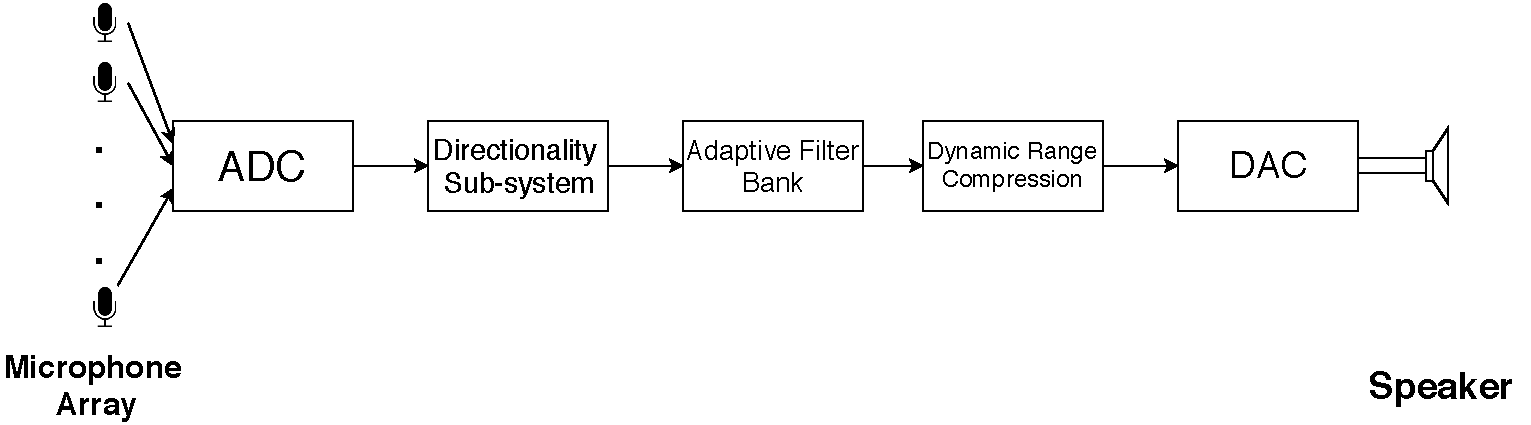
\includegraphics[width=0.9\linewidth]{system.pdf}
\caption{Overall System Block Diagram}
\label{fig:system}
\end{figure}  

\section{Adaptive Filter Design}

\noindent The adaptive filter is a filter bank which consists of an array of bandpass filters. Each of the bandpass filters operate with a particular frequency range and gain. The filter bank is adaptive in the sense that the filter parameters can be adjusted by the audiologist to meet a specific requirement. This design subsection aims to utilise a frequency bank to meet an audiologists prescription.  The audiogram considered in this design is presented in Section \ref{sec:audiogram}.\\

\noindent \textbf{Approach:} Research proved that there are multiple filter bank types used to rectifying a patients audiogram, typically categorised as uniform and non-uniform. To determine the optimum design, each of these systems will be considered. Sections \ref{sec:uniDesign}, \ref{sec:symmDesign}, \ref{sec:critDesign} and \ref{sec:octDesign} present the design of the uniform, symmetric, critical-like and octave filter banks respectively. These designs will also be compared to the ANSI S1.11 specification presented in Section \ref{sec:ansi}. The directionality sub-system relies on the phase response of the system and thus, only \textit{FIR} filters (because of their linear phase characteristics) will be considered as oppose to \textit{IIR} filters. Furthermore, because \textit{FIR} filters are stable, an accurate behaviour of the filter bank can be simulated and predicted. Two metrics are used to measure a filter banks performance namely; matching error and group delay. The matching error is defined as the difference between the filter bank response and the perscription. The group delay $(T_g)$ is calculated as shown in equation \ref{eqn:grpDelay} \cite{chang}.

\begin{equation}
\label{eqn:grpDelay}
T_g = \frac{P}{2f_s}
\end{equation}

\noindent $P$ is the order corresponding to the filter which bottlenecks the filter bank (i.e. the filter with the highest order) and $f_s$ is the sampling frequency. Both metrics are considered when choosing a filter bank design.

\subsection{Audiogram}
\label{sec:audiogram}

\noindent The audiogram considered in this design corresponds to a patient with conductive hearing loss. Audiologists typically measure a patients hearing at $125Hz$, $250Hz$, $500Hz$, $1kHz$, $2kHz$, $4kHz$ and $8kHz$ \cite{mahmoud}. \texttt{MATLAB}'s \texttt{pchip} function was used to interpolate these values to provide hearing threshold values for the full $20Hz$ to $8kHz$ range. Reference \cite{mahmoud} provides audiograms for normal hearing and conductive hearing loss. Figure \ref{fig:normCondAudio} illustrates these audiograms.

\begin{figure}[h]
\centering
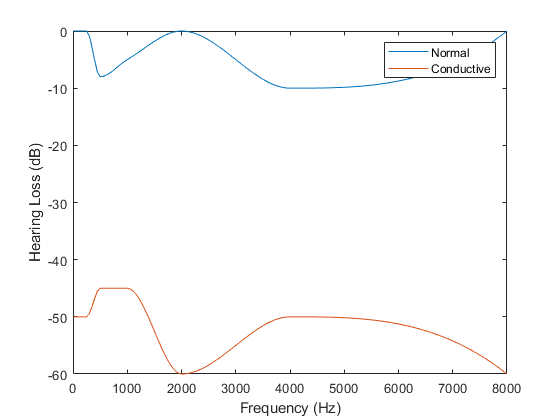
\includegraphics[width=0.6\linewidth]{normCondAudiogram.PNG}
\caption{Audiogram for Normal Hearing and Conductive Hearing Loss}
\label{fig:normCondAudio}
\end{figure}  

\noindent The filter bank aims match the conductive hearing loss patients audiogram to the normal hearing audiogram.

\subsection{Insertion Gain}
\label{sec:insertGain}

\noindent The filter bank corrects the audiogram by applying gain to particular frequencies sub-bands. Each sub-band gain is defined as insertion gain. The accuracy of the filter bank is based on it's ability to match the prescription formula. Therefore, the prescription formula is considered to be a black box and as a result, the performance of the filter bank is independent of the prescription formula used. For simplicity, this design calculates the insertion gain using the NAL-R formulas given in equation \ref{eqn:nalRp}.

\begin{equation}
\label{eqn:nalRp}
\begin{aligned}
H_{3FA} &= (H_{500} + H_{1k} + H_{2k})/3 \\
IG_i &= 0.15 \times H_{3FA} + (0.31\times H_i) + k_i
\end{aligned}
\end{equation}

\noindent Where $IG_i$ is the insertion gain, $H_i$ is the audiogram value at the $i^{th}$ sampled frequency and $k_i$ is a constant at the $i^{th}$ sampled frequency given by Table \ref{tab:kiVal} in Appendix \ref{app:insertGainParam}. Similarly to the audiogram, the insertion gain values were interpolated using \texttt{MATLAB's} \texttt{pchip} function. The insertion gains for the full frequency range is illustrated in Figure \ref{fig:igFreqRange}. 

\begin{figure}[h]
\centering
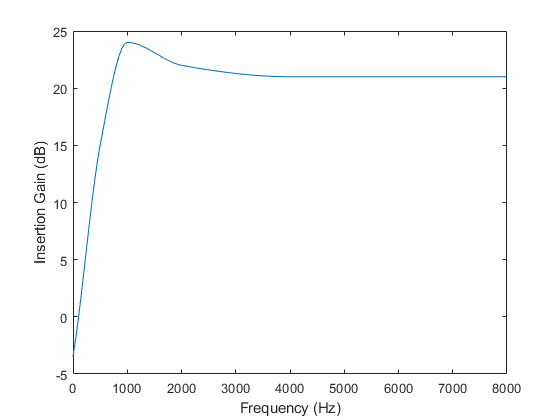
\includegraphics[width=0.6\linewidth]{igFreqRange.PNG}
\caption{Interpolated Insertion Gain for Full Frequency Range}
\label{fig:igFreqRange}
\end{figure}  

\noindent A sub-band's insertion gain is taken as the average insertion gain within the sub-band range.

\subsection{Number of Filters} 
\label{sec:numFreqBands}

\noindent As stated above, the filter bank consists of multiple bandpass filters, each operating over a specific sub-band. Therefore, the number of filters used must be investigated; particularly for the uniform, critical-like, symmetric and octave filter banks designs. A uniform filter bank was used to investigate the effect that increasing the number of filters has on matching error and computational complexity. Appendix \ref{app:numFilt} provides the details of the filter banks used in this investigation. Figure \ref{fig:numBandsErrorFreq} and \ref{fig:numBandsErrorBand} illustrate the matching error for each band across the frequency range and the mean error for each number of frequency bands respectively.

\begin{figure}
\centering
\begin{minipage}{.45\linewidth}
  \centering
  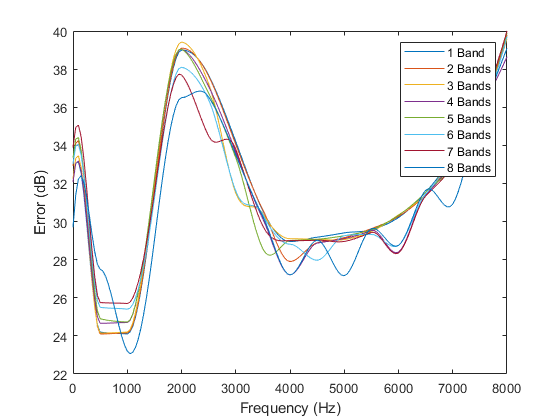
\includegraphics[width=0.9\linewidth]{numBandsErrorFreq.png}
  \captionof{figure}{Matching Error Across Frequency Spectrum per Filter Bank}
  \label{fig:numBandsErrorFreq}
\end{minipage}%
\begin{minipage}{.45\linewidth}
  \centering
  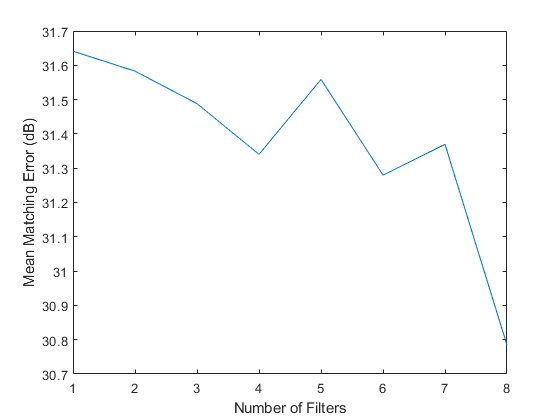
\includegraphics[width=0.9\linewidth]{numBandErrorBand.png}
  \captionof{figure}{Mean Matching Error per Filter Bank}
  \label{fig:numBandsErrorBand}
\end{minipage}
\end{figure}

\noindent Figure \ref{fig:numBandsErrorBand} illustrates that increasing the number of bands, decreases the mean matching error. This is because increasing the number of filters emphasises the frequency sub-bands that need to be adjusted. Therefore, the design should aim to maximise the number of filters.

\subsection{Uniform, Critical-like, Symmetric and Octave Filter Bank Design}
\label{sec:uniCritSymOct}

\noindent This section aims to optimise the structure of the filter bank's frequency bands. Therefore, a comparison between a uniform, symmetric, critical-like and octave filter banks will be made. These filters will then be compared to the ANSI S1.11 filter bank. To draw a fair comparison, all of the filters will be design with the parameters given in Table \ref{tab:numFilt_FiltSpec} in Appendix \ref{app:numFilt}. Each filter bank will consist of $8$ bandpass filters. Initially, the transition band per sub-band is set to $10\%$ of the sub-band's bandwidth. However, through simulation, it was found that adjusting the transition bandwidth significantly affected the performance. Therefore, each sub-band's transition bandwidth is iteratively adjusted to achieve the optimal performance. This allows for the best performing filter banks to be compared. Therefore, concrete performance decisions can be made. The same insertion gain method as in Section \ref{sec:insertGain} will be used.

\subsubsection{Uniform Filter Bank Design}
\label{sec:uniDesign}

\noindent A uniform filter bank consist of an array of evenly spaced, filters with equal bandwidths \cite{chang}. Uniform filter banks are simple and easy to implement. However, for a sufficient resolution, uniform filter banks requires more bands than non-uniform filter banks for a good fit. The additional filters implies that more computations are required and thus, the filter bank's group delay is potentially increased \cite{brennan}. This design optimised Section \ref{sec:numFreqBands}'s $8$ sub-band design by adjusting the filter bands to minimise aliasing effects. The filter bank characteristics are given in Table \ref{tab:uniFiltSpec} of Appendix \ref{app:uniFreqBand}. This design achieved and average and maximum matching error of $1.36dB$ and $11.25dB$ respectively with a group delay of $5.48ms$. The matching error across the full frequency spectrum can be seen in Figure \ref{fig:uniMatErr} of Appendix \ref{app:uniFreqBand}.

\subsubsection{Symmetric Filter Bank Design}
\label{sec:symmDesign}

\noindent Symmetric filter banks provde an improvement on the uniform filter bank. The non-uniform sub-bands are symmetric about the center frequency of the frequency spectrum, in this case $4kHz$. Symmetric filter banks have the ability of enhancing the matching error of low and high, or mid frequencies \cite{sebastian}. Figure \ref{fig:normCondAudio} illustrates that the threshold of a conductive hearing loss patient is worse at the low and high frequencies. Therefore, the frequency bands will be chosen such that these frequencies are emphasised. Table \ref{tab:symFreqBand} in Appendix \ref{app:symFreqBands} illustrates the bands used in this investigation. Simulation illustrated that the symmetric filter bank achieved an average error of $1.34dB$ with a maximum matching error of $9.4dB$. This filter bank achieved a group delay of $14.92ms$. The matching error for the full frequency spectrum is illustrated in Figure \ref{fig:symMatErr} in Appendix \ref{app:symFreqBands}.


\subsubsection{Critical-like Filter Bank Design}
\label{sec:critDesign}

\noindent This filter is forms part of the non-uniform filter bank category. This filter design attempts to account for the psychoacoustic characteristics using the critical bands of the Bark Scale \cite{chong}. Table \ref{tab:bark} in Appendix \ref{app:bark} provides the Bark scale's critical frequency band information. This investigation is limited to using $8$ filters and a maximum frequency of $8kHz$. Therefore, the sub-bands are set as shown in Table \ref{tab:critFiltFreqBand} of Appendix \ref{app:critFiltFreqBand}.	This design achieved an average and maximum matching error of $0.87dB$ and $8.15dB$ respectively and a group delay of $16.18ms$. The matching error for the full frequency spectrum is illustrated in Figure \ref{fig:critMatErr} of Appendix \ref{app:critFiltFreqBand}.


\subsubsection{Octave Filter Bank Design}
\label{sec:octDesign}

\noindent As stated above, separating a frequency spectrum into octaves allows for the quality of sound to be measure and by derivative, improved \cite{octave}. It is therefore natural for a filter bank to be designed using this principle. Each filter bank sub-band will have a center frequency relative to the reference sub-band center frequency $f_c [0] = 1000Hz$ \cite{octFreqCalc}. The center frequency of each sub-band is calculated using equation \ref{eqn:octCentFreq}. The corresponding upper $(f_{cu})$ and lower $(f_{cl})$ passband frequencies are calculated using equation \ref{eqn:octFreqEdge} \cite{octFreqCalc}.
%
\begin{equation}
\label{eqn:octCentFreq}
f_c[k-1] = f[k]/2 
\end{equation}
\begin{equation}
\begin{aligned}
\label{eqn:octFreqEdge}
f_{cu}[k] &= \frac{f_c[k] }{2^{1/2}}\\
f_{cl}[k] &= 2^{1/2}\times f_c[k]
\end{aligned}
\end{equation}
%

\noindent The center frequencies for this filter bank are chosen to be $63Hz$, $125Hz$, $250Hz$, $500Hz$, $1kHz$, $2kHz$, $4kHz$ and $8kHz$ which results in the filter specifications given in Table \ref{tab:octFreqBands} of Appendix \ref{app:octFreqBands}. Simulations demonstrated that this filter bank achieved an average and maximum matching error of $0.72dB$ and $10.44dB$ respectively. Figure \ref{fig:octMatErr} in Appendix \ref{app:octFreqBands} illustrates the matching error across the full frequency spectrum. The group delay for this filter was $37.45ms$.

\subsection{ANSI S1.11 Design}
\label{sec:ansi}

\noindent A octave filter bank was designed using the ANSI S1.11 specficiations. The class $2$ attenuation specification is chosen for two reasons. The first being that as it allows a $1dB$ ripple which allows for an accurate comparison with the aforementioned filter banks. Secondly, the larger ripple decreases the delay \cite{yang}. The stop band attenuation is set to $60dB$. This is considered to be sufficient for hearing loss applications \cite{ansiAtten}. ANSI S1.11 compliant filter banks are typically implemented using $IIR$ filters. However, for an accurate comparison, this investigation implements the ANSI S1.11 standard using $FIR$ filters. The frequency specifications are calculated as shown in Appendix \ref{app:ansiSpec} with the resulting specifications summarised in Table \ref{tab:ansiFreqSpec} of Appendix \ref{app:ansiSpec}. Through simulation, the mean matching error was $0.25dB$ and the maximum error was $2.3dB$. The ANSI S1.11 filter bank achieved a group delay of $47.28ms$. Figure \ref{fig:ansiOctMatErr} in Appendix \ref{app:ansiSpec} illustrates the matching error across the full frequency spectrum.



\subsection{Filter Design Selection}
\label{sec:filtSelect}

\noindent From the several investigated filter bank designs, the optimal design must be chosen. This decision is based on two metrics; namely matching error performance and computational complexity. Figure \ref{fig:matErrDelay} illustrates the matching error and computational complexity of each design.

\begin{figure}[h]
\centering
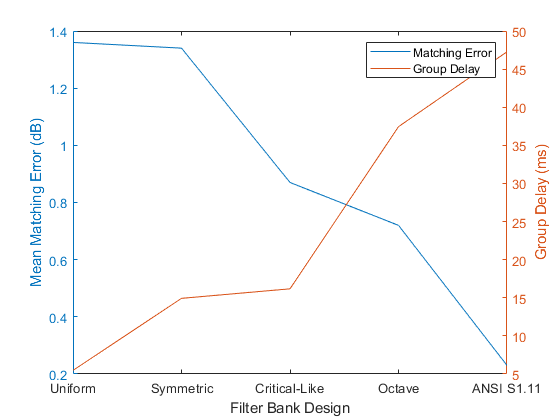
\includegraphics[width=0.6\linewidth]{matErrDelay.PNG}
\caption{Mean Matching Error and Group Delay for each Filter Bank Design}
\label{fig:matErrDelay}
\end{figure}

\noindent From Figure \ref{fig:matErrDelay}, the critical-like and octave filter banks provide the best balance between matching error and group delay. However, experimentation found that only slight optimisations can be applied to these filter banks. The ANSI S1.11 has a significantly lower matching error compared to the other filter banks. Furthermore, the group delay of the ANSI S1.11 filter bank can be significantly optimised by using transition bandwidth relaxation (adjusting the transition bandwidth to reduce the filter order) \cite{chang}. Therefore, the ANSI S1.11 filter bank design technique is chosen to design the adaptive filter bank. The optimisations applied to this filter bank are presented in Section \ref{sec:filtBankOpt}.

\subsection{Filter Bank Optimisation}
\label{sec:filtBankOpt}

\noindent In the previous section, the investigations were constrained to using 8 filters. ANSI S1.11 provides specifications for $1/3$-octave filter banks, meaning there are $3$ sub-bands per octave. As shown in Section \ref{sec:numFreqBands}, increasing the number of sub-bands decreases the matching error. A design was simulated using the frequency sub-bands $F_{14} \rightarrow F_{39}$ from the ANSI S1.11 specification. Simulations revealed extensive aliasing affects and a maximum group delay of $107.7ms$. This is unacceptable. Relaxation techniques exist to reduce rigidity of the ANSI S1.11 specification by increasing the relevant transition bandwidths. However, the lowest frequency sub-band $(F_{14})$ has a lower passband frequency of $23Hz$. However, it is impossible to make the lower transition bandwidth large enough to reduce the order without reducing the attenuation. Therefore, the octave filter bank is chosen over the $1/3$-octave filter bank.\\
\newline
\noindent As shown in Section \ref{sec:filtSelect}, the ANSI S1.11 octave filter bank is highly accurate, but has an unacceptably large group delay. Therefore, the ANSI S1.11 octave filter bank will be optimised to meet the $10ms$ group delay requirement. As seen in equation \ref{eqn:grpDelay}, the group delay is dependant on the filter order. The maximum filter order to achieve a group delay of $10ms$ is therefore, $P = (10ms)\times (2f_s) = 400$. Using \texttt{MATLAB's} Park-McClennan algorithm function \texttt{firpmord}, it was found that the first, second and third sub-band filters did not meet this requirement with filter orders of $1350$, $1890$ and $945$ respectively. To reduce the order and hence the group delay, relaxation of the ANSI S1.11 specifications can be applied. Using iterative techniques, it was found that a transition bandwidth of $75Hz$ yields a $10ms$ group delay. The filter bank will be bottlenecked by the filter with the maximum group delay. Therefore, the minimum transition bandwidth is set at $80Hz$ to ensure a group delay $<10ms$ per filter. The first passband frequency of the ANSI S1.11 filter bank designed in Section \ref{sec:ansi} was $22Hz<80Hz$. Therefore, the selected sub-bands per octave were adjusted such that the first passband frequency could meet the $10ms$ group delay requirement. Table \ref{tab:ansiOptSpec} in Appendix \ref{app:ansiOptSpec} illustrate the adjusted frequency specifications. The adjusted filter bank yielded a maximum group delay of $8.88ms$ with a mean and maximum matching error of $0.83dB$ and $10.42dB$ respectively. The matching error for the full frequency spectrum is illustrated in Figure \ref{fig:ansiOptMatErr} of Appendix \ref{app:ansiOptSpec}. 


\section{Dynamic Range Compression Design}
\label{sec:dynamicCompress}

\noindent This section aims to design a compression algorithm to maintain the output of the filter bank within a comfortable auditory range. Figure \ref{fig:loud} illustrates the loudness range that normal and hearing impaired people can hear, and is comfortable. 

\begin{figure}[h]
\centering
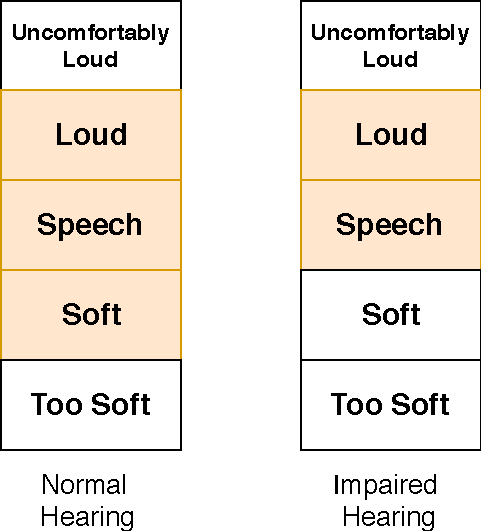
\includegraphics[width=0.35\linewidth]{loud.pdf}
\caption{Comfortable Loudness Range for Normal and Hearing Impaired People}
\label{fig:loud}
\end{figure} 

\noindent As seen from Figure \ref{fig:loud}, speech is perceived as soft to a hearing impaired individual. Therefore, by merely amplifying the sound to improve speech perception, loud sounds that were once comfortable will be shifted into the uncomfortable region. Dynamic range compression ensures the the output of the filter bank remains in a comfortable auditory region by compressing the loudness range into the loudness range, audible range to the patient. The design of the dynamic range compression component involves choosing suitable values for the compression threshold, compression ratio, attack and release times and the number of channels. More information about these parameters can be found in Appendix \ref{app:compressPara}. The parameters chosen for this design are such that speech intelligibility is maximised. The compression threshold should be set below $50dBSPL$ to amplify the soft speech into an audible range \cite{compressHand}. In this design, the compression threshold is set at $30dBSPL$. To operate over a wide input range, the compression recommended to be below $4$ and therefore, is set at $3$ in this design. The attack and release times are set at \texttt{MATLAB's} recommended $0.05s$ and $0.2s$ respectively. Each of the sub-band filter banks will be followed by a dynamic range compressor. This is chosen to improve speed intelligibility by amplifying the loud vowel sounds separately from the softer consonant sounds. The dynamic range compressor output is calculated as shown in Appendix \ref{app:compressCalc}. To test this algorithm, gain was applied to a $6kHz$ digital sine wave with an amplitude of $1$ before it was passed through the compressor. By adjusting the gain, the affect of the compressor can be seen which is referred to as the static characteristics. Figure \ref{fig:staticChar} illustrates the static characteristics for dynamic range compressor used in this design.

\begin{figure}[h]
\centering
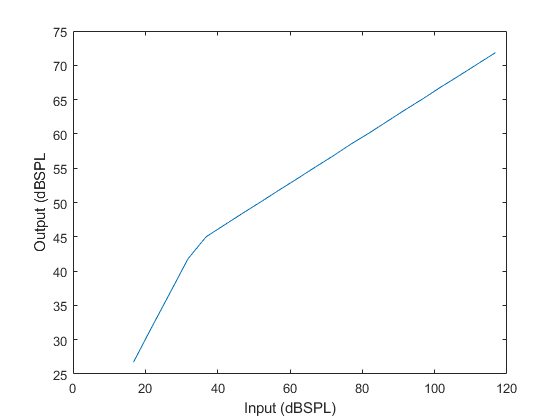
\includegraphics[width=0.6\linewidth]{staticChar.PNG}
\caption{Dynamic Range Compressor Static Characteristics}
\label{fig:staticChar}
\end{figure}

\section{System Realisation}

\noindent This subsystem consists of an input, an analysis and synthesis stage, and finally an output. For the analysis stage, a DSP\footnote{Digital-Signal-Processor} is required which will house the filter bank and the dynamic range compression algorithm. The sythesis stage consists of a DAC, reconstruction filter, pre-amplifier which outputs to a speaker.  TALK ABOUT THE INPUT. The Analog Devices, \textit{ADAU1463 Sigma Digital Audio Processor} is chosen as the DSP for this system. This DSP can handle $24000$ filter taps per sample \cite{dsp}. The optimised filter bank consists of a total of $1683$ filter taps per sample and therefore, this DSP can easily handle the filter bank processing requirements. The \textit{ADAU1463} has $2$ communication port types, $I^2C$ and $SPI$.  To synthesise the signal, the output of the DSP is connected to the \textit{TLV320AIC3109-Q1} audio processor. The \textit{ADAU1463} supports both $SPI$ and $I^2C$ as opposed to \textit{TLV320AIC3109-Q1} which only supports $I^2C$. Therefore, the \textit{ADAU1463} communicates with the \textit{TLV320AIC3109-Q1} via the $I^2C port$. The \textit{TLV320AIC3109-Q1} contains the DAC, reconstruction filter and pre-amplifier suitable for a $16 \Omega$ headphone output load resistance \cite{dac}. The \textit{CE20M-16} micro speaker is specified to output the sound of the system to the patient. The \textit{CE20M-16} micro speaker has a $16 \Omega$ load resistance \cite{speaker} and thus, is suitable for the output of the \textit{TLV320AIC3109-Q1} audio processor. An overall circuit diagram is giving in Figure XXX of Appendix XXX.


\section{Success Criterion}

\noindent To deem this subsystem successful, the adaptive filter bank and dynamic range compression must be combined and simulated. The results of these simulations should be compared to that of the design requirements and constraints.  The following criterion will be used to measure the success of each subsystem.

\begin{enumerate}
	\item Matching Error: In the previous section, the entire frequency spectrum was analysed. The most common frequency range of conversation however, is $500Hz$ to $4kHz$ with particular importance at $2kHz$ \cite{speechDPA}. Therefore, since the focus of this design is maximise speech intelligibility, the matching error between $500Hz$ and $4kHz$ will determine the success of the frequency response matching component.
	\item System Response: As stated above, the response time of the system is a critical design consideration. Since the directionality is assumed to have a response time of $10ms$, the overall response time of this subsection cannot exceed $10ms$ to meet the $20ms$ response time requirement.
	\item Loudness Compression: The dynamic range compression must ensure that sounds, comfortable to the human ear, remain in the comfortable loudness region $(40dBSPL \rightarrow 80dBSPL)$ \cite{loudRange}.
\end{enumerate}


\section{Testing and Critical Evaluation of Results}

\noindent Simulations were performed on the combined subsystem. The measurements taken from these simulations were compared to the success criteria of the subsystem. The matching error, group delay and dynamic range compression results are provide in Section \ref{sec:resMatErr}, \ref{sec:resGroupDelay} and \ref{sec:resCompress} respectively. A technical view point regarding this design is presented in Section \ref{sec:socioImpacts} with a non-technical discussion presented in Appendix \ref{app:nonTech}.
 
	\subsection{Matching Error Results}
\label{sec:resMatErr}

\noindent The optimised filter bank has a mean and maximum matching of $0.73dB$ and $4.5dB$ respectively between $500Hz$ and $4kHz$. Whilst the average matching error falls within the $3dB$ constraint, the maximum error does not. When the transition bandwidths are adjusted, the impact of aliasing is increased. As a result, when the filters are combined, the overall response deviates further from the desired response and thus, the matching error increases. In terms of matching error, the ideal filter bank would be constructed of ideal filters as no aliasing would occur.

\subsection{Group Delay Results}
\label{sec:resGroupDelay}


\subsection{Dynamic Range Compression Results}
\label{sec:resCompress}



\subsection{Socioeconomic Impacts of Design}
\label{sec:socioImpacts}




\section{Future Recommendations}

why you dont use multirate filters\\
divide into what needs to be improved and what the implementation considerations must be
\section{Conclusion}

\section*{Acknowledgements}

\noindent I would like to take this opportunity to thank Prof. Rubin for all of his help and assistance with this project. A special thanks to the University of the Witwatersrand and all of the staff that were involved in the development of this project.

\newpage
\printbibliography
\newpage
\begin{appendices}

\section{Impact Appendix - Non-Technical thing}
\label{app:nonTech}

\section{Insertion Gain Parameters}
\label{app:insertGainParam}

\noindent The values of $k_i$ is determined by Table \ref{tab:kiVal}.

% Table generated by Excel2LaTeX from sheet 'Insertion Gain ParametersFre'
\begin{table}[htbp]
  \centering
  \caption{$k_i$ Parameter at Specific Frequency Values}
    \begin{tabular}{|l|r|r|r|r|r|r|r|}
    \hline
    \textbf{Frequency (Hz)} & 250   & 500   & 1000  & 2000  & 3000  & 4000  & 6000 \\
    \hline
    \textbf{$k_i (dB)$} & -17   & -8    & 1     & -1    & -2    & -2    & -2 \\
    \hline
    \end{tabular}%
  \label{tab:kiVal}%
\end{table}%


\section{Number of Filters Investigation}
\label{app:numFilt}

\noindent In this investigation, a filter bank was constructed. Each filter was designed using \texttt{Simulink's} digital bandpass filter. The design settings used are given in Table \ref{tab:numFilt_FiltSpec}.

% Table generated by Excel2LaTeX from sheet 'Sheet1'
\begin{table}[htbp]
  \centering
  \caption{Filter Design Settings}
  
    \begin{tabular}{|l|l|}
    \hline
    Impulse Response  & FIR  \\
    \hline
    Order Mode & Minimum \\
    \hline
    Filter Type & Single-rate \\
    \hline
    Input Sample Rate & $20kHz$ \\
    \hline
    Passband ripple & $1dB$ \\
    \hline
    Transition Bandwidth & $200Hz$ \\
    \hline
    Design Method & Equiripple \\
    \hline
    Structure  & Direct-form FIR \\
    \hline
    \end{tabular}%
  \label{tab:numFilt_FiltSpec}%
\end{table}%

\noindent The order of an FIR filter corresponds to the window length. Therefore, it is set to a minimum to keep the results consistent. Tables \ref{tab:filtPara1Band} to \ref{tab:filtPara8Band} provide the filter range and gains used in this investigation. $f_{s1}$, $f_{p1}$, $f_{p2}$ and $f_{s2}$ correspond to the lower stopband frequency, the lower pass band frequency, the upper passband frequency and the upper stopband frequency respectively. $A_{s1}$ and $A_{s2}$ correspond to the lower and upper stopband attenuations.

% Table generated by Excel2LaTeX from sheet 'Sheet1'
\begin{table}[htbp]
  \centering
  \caption{Filter Parameters - 1 Band}
    \begin{tabular}{|l|l|}
    \hline
    \textbf{Parameter} & \textbf{Filter 1} \\
    \hline
    $f_{s1} (Hz)$   & \multicolumn{1}{r|}{$20$} \\
    \hline
    $f_{p1} (Hz)$   & \multicolumn{1}{r|}{$250$} \\
    \hline
    $f_{p2} (Hz)$   & \multicolumn{1}{r|}{$8000$} \\
    \hline
    $f_{s2} (Hz)$   & \multicolumn{1}{r|}{$8200$} \\
    \hline
    $A_{s1} (dB)$   & $G1dB + 3$ \\
    \hline
    $A_{s2} (dB)$   & $G1dB + 3$ \\
    \hline
    \end{tabular}%
  \label{tab:filtPara1Band}%
\end{table}%


% Table generated by Excel2LaTeX from sheet 'Sheet1'
\begin{table}[htbp]
  \centering
  \caption{Filter Parameters - 2 Bands}
    \begin{tabular}{|l|l|l|}
    \hline
    \textbf{Parameter} & \textbf{Filter 1} & \textbf{Filter 2} \\
    \hline
    $f_{s1} (Hz)$   & \multicolumn{1}{r|}{$20$} & \multicolumn{1}{r|}{$ 3800$ } \\
    \hline
    $f_{p1} (Hz)$  & \multicolumn{1}{r|}{$250$} & \multicolumn{1}{r|}{$4000$} \\
    \hline
    $f_{p2} (Hz)$   & \multicolumn{1}{r|}{$ 4000$ } & \multicolumn{1}{r|}{$8000$} \\
    \hline
    $f_{s2} (Hz)$   & \multicolumn{1}{r|}{$ 4200$ } & \multicolumn{1}{r|}{$8200$} \\
    \hline
    $A_{s1} (dB)$   & $G1dB + 3$ & $G1dB + G2dB + 3$ \\
    \hline
    $A_{s2} (dB)$   & $G1dB + G2dB + 3$ & $G2dB + 3$ \\
    \hline
    \end{tabular}%
  \label{tab:filtPara2Band}%
\end{table}%

% Table generated by Excel2LaTeX from sheet 'Sheet1'
\begin{table}[htbp]
  \centering
  \caption{Filter Parameters - 3 Bands}
    \begin{tabular}{|l|l|l|l|}
    \hline
    \textbf{Parameter} & \textbf{Filter 1} & \textbf{Filter 2} & \textbf{Filter 3} \\
    \hline
    $f_{s1} (Hz)$   & \multicolumn{1}{r|}{$ 20$ } & \multicolumn{1}{r|}{$ 2800$ } & \multicolumn{1}{r|}{$ 5550$ } \\
    \hline
    $f_{p1} (Hz)$   & \multicolumn{1}{r|}{$ 250$ } & \multicolumn{1}{r|}{$ 3000$ } & \multicolumn{1}{r|}{$ 5750$ } \\
    \hline
    $f_{p2} (Hz)$   & \multicolumn{1}{r|}{$ 3000$ } & \multicolumn{1}{r|}{$ 5750$ } & \multicolumn{1}{r|}{$ 8000$ } \\
    \hline
    $f_{s2} (Hz)$   & \multicolumn{1}{r|}{$ 3200$ } & \multicolumn{1}{r|}{$ 5950$ } & \multicolumn{1}{r|}{$ 8200$ } \\
    \hline
    $A_{s1} (dB)$   &$  G1dB + 3$  & $ G1dB + G2dB + 3$  & $ G2dB + G3dB + 3$  \\
    \hline
    $A_{s2} (dB)$   & $ G1dB + G2dB + 3$  & $ G2dB + G3dB + 3 $ & $ G3dB + 3$  \\
    \hline
    \end{tabular}%
  \label{tab:filtPara3Band}%
\end{table}%


% Table generated by Excel2LaTeX from sheet 'Sheet1'
\begin{table}[htbp]
  \centering
  \caption{Filter Parameters - 4 Bands}
  \begin{adjustbox}{width=0.9\linewidth}
    \begin{tabular}{|l|l|l|l|l|}
    \hline
    \textbf{Parameter} & \textbf{Filter 1} & \textbf{Filter 2} & \textbf{Filter 3} & \textbf{Filter 4} \\
    \hline
    $f_{s1} (Hz)$   & \multicolumn{1}{r|}{$20$} & \multicolumn{1}{r|}{$1800$} & \multicolumn{1}{r|}{$3800$} & \multicolumn{1}{r|}{$5800$} \\
    \hline
    $f_{p1} (Hz)$   & \multicolumn{1}{r|}{$250$} & \multicolumn{1}{r|}{$2000$} & \multicolumn{1}{r|}{$4000$} & \multicolumn{1}{r|}{$6000$} \\
    \hline
    $f_{p2} (Hz)$   & \multicolumn{1}{r|}{$2000$} & \multicolumn{1}{r|}{$4000$} & \multicolumn{1}{r|}{$6000$} & \multicolumn{1}{r|}{$8000$} \\
    \hline
    $f_{s2} (Hz)$   & \multicolumn{1}{r|}{$2200$} & \multicolumn{1}{r|}{$4200$} & \multicolumn{1}{r|}{$6200$} & \multicolumn{1}{r|}{$8200$} \\
    \hline
    $A_{s1} (dB)  $ &$ G1dB + 3 $&$ G1dB + G2dB + 3 $&$ G2dB + G3dB + 3$ & $G3dB + G4dB + 3$ \\
    \hline
    $A_{s2} (dB)$   & $G1dB + G2dB + 3$ & $G2dB + G3dB + 3 $& $G3dB + G4dB + 3$ &$ G4dB + 3 $\\
    \hline
    \end{tabular}%
    \end{adjustbox}
  \label{tab:filtPara4Band}%
\end{table}%

% Table generated by Excel2LaTeX from sheet 'Sheet1'
\begin{table}[htbp]
  \centering
  \caption{Filter Parameters - 5 Bands}
  \begin{adjustbox}{width=0.9\linewidth}
    \begin{tabular}{|l|l|l|l|l|l|}
    \hline
    \textbf{Parameter} & \textbf{Filter 1} & \textbf{Filter 2} & \textbf{Filter 3} & \textbf{Filter 4} & \textbf{Filter 5} \\
    \hline
    $f_{s1} (Hz)$   & \multicolumn{1}{r|}{$20$} & \multicolumn{1}{r|}{$1700$} & \multicolumn{1}{r|}{$3350$} & \multicolumn{1}{r|}{$5000$} & \multicolumn{1}{r|}{$6650$} \\
    \hline
    $f_{p1} (Hz)$   & \multicolumn{1}{r|}{$250$} & \multicolumn{1}{r|}{$1900$} & \multicolumn{1}{r|}{3550} & \multicolumn{1}{r|}{$5200$} & \multicolumn{1}{r|}{$6850$} \\
    \hline
    $f_{p2} (Hz)$   & \multicolumn{1}{r|}{$1900$} & \multicolumn{1}{r|}{$3550$} & \multicolumn{1}{r|}{$5200$} & \multicolumn{1}{r|}{$6850$} & \multicolumn{1}{r|}{$8000$} \\
    \hline
    $f_{s2} (Hz)$   & \multicolumn{1}{r|}{1100} & \multicolumn{1}{r|}{$3750$} & \multicolumn{1}{r|}{$5400$} & \multicolumn{1}{r|}{$7050$} & \multicolumn{1}{r|}{$8200$} \\
    \hline
    $A_{s1} (dB)$   &$ G1dB + 3 $& $G1dB + G2dB + 3 $& $G2dB + G3dB + 3$ &$ G3dB + G4dB + 3 $& $G4dB + G5dB + 3$ \\
    \hline
    $A_{s2} (dB)$   & $G1dB + G2dB + 3 $&$ G2dB + G3dB + 3 $&$ G3dB + G4dB + 3$ &$ G4dB + G5dB + 3$ &$ G5dB + 3$ \\
    \hline
    \end{tabular}%
    \end{adjustbox}
  \label{tab:filtPara5Band}%
\end{table}%

% Table generated by Excel2LaTeX from sheet 'Sheet1'
\begin{table}[htbp]
  \centering
  \caption{Filter Parameters - 6 Bands}
  \begin{adjustbox}{width=0.9\linewidth}
    \begin{tabular}{|l|l|l|l|l|l|l|}
    \hline
    \textbf{Parameter} & \textbf{Filter 1} & \textbf{Filter 2} & \textbf{Filter 3} & \textbf{Filter 4} & \textbf{Filter 5} & \textbf{Filter 6} \\
    \hline
    $f_{s1} (Hz)$   & \multicolumn{1}{r|}{$20$} & \multicolumn{1}{r|}{$1300$} & \multicolumn{1}{r|}{$2800$} & \multicolumn{1}{r|}{$4300$} & \multicolumn{1}{r|}{$5800$} & \multicolumn{1}{r|}{$7300$} \\
    \hline
    $f_{p1} (Hz)$   & \multicolumn{1}{r|}{$250$} & \multicolumn{1}{r|}{$1500$} & \multicolumn{1}{r|}{$3000$} & \multicolumn{1}{r|}{$4500$} & \multicolumn{1}{r|}{$6000$} & \multicolumn{1}{r|}{$7500$} \\
    \hline
    $f_{p2} (Hz)$   & \multicolumn{1}{r|}{$1500$} & \multicolumn{1}{r|}{$3000$} & \multicolumn{1}{r|}{$4500$} & \multicolumn{1}{r|}{$6000$} & \multicolumn{1}{r|}{$7500$} & \multicolumn{1}{r|}{$8000$} \\
    \hline
    $f_{s2} (Hz)$   & \multicolumn{1}{r|}{$1700$} & \multicolumn{1}{r|}{$3200$} & \multicolumn{1}{r|}{$4700$} & \multicolumn{1}{r|}{$6200$} & \multicolumn{1}{r|}{$7700$} & \multicolumn{1}{r|}{$8200$} \\
    \hline
    $A_{s1} (dB)$   & $G1dB + 3$ & $G1dB + G2dB + 3 $& $G2dB + G3dB + 3 $&$ G3dB + G4dB + 3$ &$ G4dB + G5dB + 3$ &$ G5dB + G6dB + 3$ \\
    \hline
    $A_{s2} (dB)$   &$ G1dB + G2dB + 3$ &$ G2dB + G3dB + 3$ & $G3dB + G4dB + 3$ & $G4dB + G5dB + 3$ & $G5dB + G6dB + 3 $& $G6dB + 3$ \\
    \hline
    \end{tabular}%
    \end{adjustbox}
  \label{tab:filtPara6Band}%
\end{table}%


% Table generated by Excel2LaTeX from sheet 'Sheet1'
\begin{table}[htbp]
  \centering
  \caption{Filter Parameters - 7 Bands}
  \begin{adjustbox}{width=0.9\linewidth}
    \begin{tabular}{|l|l|l|l|l|l|l|l|}
    \hline
    \textbf{Parameter} & \textbf{Filter 1} & \textbf{Filter 2} & \textbf{Filter 3} & \textbf{Filter 4} & \textbf{Filter 5} & \textbf{Filter 6} & \textbf{Filter 7} \\
    \hline
    $f_{s1} (Hz)$   & \multicolumn{1}{r|}{$20$} & \multicolumn{1}{r|}{$1200$} & \multicolumn{1}{r|}{$2350$} & \multicolumn{1}{r|}{$3500$} & \multicolumn{1}{r|}{$4650$} & \multicolumn{1}{r|}{$5800$} & \multicolumn{1}{r|}{$6950$} \\
    \hline
    $f_{p1} (Hz)$    & \multicolumn{1}{r|}{$250$} & \multicolumn{1}{r|}{$1400$} & \multicolumn{1}{r|}{$2550$} & \multicolumn{1}{r|}{$3700$} & \multicolumn{1}{r|}{$4850$} & \multicolumn{1}{r|}{$6000$} & \multicolumn{1}{r|}{$7150$} \\
    \hline
    $f_{p2} (Hz)$    & \multicolumn{1}{r|}{$1400$} & \multicolumn{1}{r|}{$2550$} & \multicolumn{1}{r|}{$3700$} & \multicolumn{1}{r|}{$4850$} & \multicolumn{1}{r|}{$6000$} & \multicolumn{1}{r|}{$7150$} & \multicolumn{1}{r|}{$8000$} \\
    \hline
    $f_{s2} (Hz)$    & \multicolumn{1}{r|}{$1600$} & \multicolumn{1}{r|}{$2750$} & \multicolumn{1}{r|}{$3900$} & \multicolumn{1}{r|}{$5050$} & \multicolumn{1}{r|}{$6200$} & \multicolumn{1}{r|}{$7350$} & \multicolumn{1}{r|}{$8200$} \\
    \hline
    $A_{s1} (dB)$   & $G1dB + 3$ &$ G1dB + G2dB + 3 $& $G2dB + G3dB + 3$ &$ G3dB + G4dB + 3$ &$ G4dB + G5dB + 3 $&$ G5dB + G6dB + 3$ &$ G6dB + G7dB + 3$ \\
    \hline
    $A_{s2} (dB)$   &$ G1dB + G2dB + 3$ &$ G2dB + G3dB + 3$ &$ G3dB + G4dB + 3$ &$ G4dB + G5dB + 3$ &$ G5dB + G6dB + 3$ &$ G6dB + G7dB + 3$ &$ G7dB + 3$ \\
    \hline
    \end{tabular}%
    \end{adjustbox}
  \label{tab:filtPara7Band}%
\end{table}%


% Table generated by Excel2LaTeX from sheet 'Sheet1'
\begin{table}[htbp]
  \centering
  \caption{Filter Parameters - 8 Banks}
  \begin{adjustbox}{width=0.9\linewidth}
    \begin{tabular}{|l|l|l|l|l|l|l|l|l|}
    \hline
    \textbf{Parameter} & \textbf{Filter 1} & \textbf{Filter 2} & \textbf{Filter 3} & \textbf{Filter 4} & \textbf{Filter 5} & \textbf{Filter 6} & \textbf{Filter 7} & \textbf{Filter 8} \\
    \hline
    $f_{s1} (Hz)$   & \multicolumn{1}{r|}{$20$} & \multicolumn{1}{r|}{$800$} & \multicolumn{1}{r|}{$1800$} & \multicolumn{1}{r|}{$2800$} & \multicolumn{1}{r|}{$3800$} & \multicolumn{1}{r|}{$4800$} & \multicolumn{1}{r|}{$5800$} & \multicolumn{1}{r|}{$6800$} \\
    \hline
    $f_{p1} (Hz)$    & \multicolumn{1}{r|}{$250$} & \multicolumn{1}{r|}{$1000$} & \multicolumn{1}{r|}{$2000$} & \multicolumn{1}{r|}{$3000$} & \multicolumn{1}{r|}{$4000$} & \multicolumn{1}{r|}{$5000$} & \multicolumn{1}{r|}{$6000$} & \multicolumn{1}{r|}{$7000$} \\
    \hline
    $f_{p2} (Hz)$    & \multicolumn{1}{r|}{$1000$} & \multicolumn{1}{r|}{$2000$} & \multicolumn{1}{r|}{$3000$} & \multicolumn{1}{r|}{$4000$} & \multicolumn{1}{r|}{$5000$} & \multicolumn{1}{r|}{$6000$} & \multicolumn{1}{r|}{$7000$} & \multicolumn{1}{r|}{$8000$} \\
    \hline
    $f_{s2} (Hz)$    & \multicolumn{1}{r|}{$1200$} & \multicolumn{1}{r|}{$2200$} & \multicolumn{1}{r|}{$3200$} & \multicolumn{1}{r|}{$4200$} & \multicolumn{1}{r|}{$5200$} & \multicolumn{1}{r|}{$6200$} & \multicolumn{1}{r|}{$7200$} & \multicolumn{1}{r|}{$8200$} \\
    \hline
    $A_{s1} (dB)$   &$ G1dB + 3$ &$ G1dB + G2dB + 3 $& $G2dB + G3dB + 3$ &$ G3dB + G4dB + 3 $&$ G4dB + G5dB + 3 $& $G5dB + G6dB + 3$ & $G6dB + G7dB + 3$ &$ G7dB + G8dB + 3$ \\
    \hline
    $A_{s2} (dB)$   &$ G1dB + G2dB + 3$ &$ G2dB + G3dB + 3$ &$ G3dB + G4dB + 3 $&$ G4dB + G5dB + 3 $& $G5dB + G6dB + 3$ &$ G6dB + G7dB + 3 $&$ G7dB + G8dB + 3$ &$ G8dB + 3 $\\
    \hline
    \end{tabular}%
    \end{adjustbox}
  \label{tab:filtPara8Band}%
\end{table}%

\section{Bark-Scale}
\label{app:bark}

\noindent Table \ref{tab:bark} provides the critical frequency bands of the Bark-scale \cite{bark}.

% Table generated by Excel2LaTeX from sheet 'Bark Scale'
\begin{table}[htbp]
  \centering
  \caption{Bark-scale Critical Frequency Bands}
    \begin{tabular}{|r|r|r|r|}
    \hline
    \multicolumn{1}{|l|}{\textbf{Number}} & \multicolumn{1}{l|}{\textbf{Center Frequency (Hz) }} & \multicolumn{1}{l|}{\textbf{Cut-Off Frequency (Hz)}} & \multicolumn{1}{l|}{\textbf{Bandwidth (Hz)}} \\
    \hline
          &       & 20    &  \\
    \hline
    1     & 60    & 100   & 80 \\
    \hline
    2     & 150   & 200   & 100 \\
    \hline
    3     & 250   & 300   & 100 \\
    \hline
    4     & 350   & 400   & 100 \\
    \hline
    5     & 450   & 510   & 110 \\
    \hline
    6     & 570   & 630   & 120 \\
    \hline
    7     & 700   & 770   & 140 \\
    \hline
    8     & 840   & 920   & 150 \\
    \hline
    9     & 1000  & 1080  & 160 \\
    \hline
    10    & 1170  & 1270  & 190 \\
    \hline
    11    & 1370  & 1480  & 210 \\
    \hline
    12    & 1600  & 1720  & 240 \\
    \hline
    13    & 1850  & 2000  & 280 \\
    \hline
    14    & 2150  & 2320  & 320 \\
    \hline
    15    & 2500  & 2700  & 380 \\
    \hline
    16    & 2900  & 3150  & 450 \\
    \hline
    17    & 3400  & 3700  & 550 \\
    \hline
    18    & 4000  & 4400  & 700 \\
    \hline
    19    & 4800  & 5300  & 900 \\
    \hline
    20    & 5800  & 6400  & 1100 \\
    \hline
    21    & 7000  & 7700  & 1300 \\
    \hline
    22    & 8500  & 9500  & 1800 \\
    \hline
    23    & 10500 & 12000 & 2500 \\
    \hline
    24    & 13500 & 15500 & 3500 \\
    \hline
    \end{tabular}%
  \label{tab:bark}%
\end{table}%

\section{Uniform Filter Bank Specifications and Results}
\label{app:uniFreqBand}

\noindent Table \ref{tab:uniFiltSpec} provides the specifications for each sub-band in the uniform filter bank.

% Table generated by Excel2LaTeX from sheet 'Uniform'
\begin{table}[htbp]
  \centering
  \caption{Uniform Filter Bank Frequency Bands}
  \begin{adjustbox}{width=0.9\linewidth}
    \begin{tabular}{|l|r|r|r|r|r|r|r|r|}
    \hline
          & \multicolumn{1}{l|}{\textbf{Filter 1}} & \multicolumn{1}{l|}{\textbf{Filter 2}} & \multicolumn{1}{l|}{\textbf{Filter 3}} & \multicolumn{1}{l|}{\textbf{Filter 4}} & \multicolumn{1}{l|}{\textbf{Filter 5}} & \multicolumn{1}{l|}{\textbf{Filter 6}} & \multicolumn{1}{l|}{\textbf{Filter 7}} & \multicolumn{1}{l|}{\textbf{Filter 8}} \\
    \hline
    \textbf{$f_{s1} (Hz)$} & 120   & 900   & 1900  & 2900  & 3900  & 4900  & 5900  & 6900 \\
    \hline
    \textbf{$f_{p1} (Hz)$} & 200   & 1000  & 2000  & 3000  & 4000  & 5000  & 6000  & 7000 \\
    \hline
    \textbf{$f_{p2} (Hz)$} & 1000  & 2000  & 3000  & 4000  & 5000  & 6000  & 7000  & 8000 \\
    \hline
    \textbf{$f_{s2} (Hz)$} & 1080  & 2100  & 3100  & 4100  & 5100  & 6100  & 7100  & 8100 \\
    \hline
    \textbf{$Gain (dB)$} & 17,16 & 23,07 & 21,62 & 21,1  & 21    & 21    & 21    & 21 \\
    \hline
    \end{tabular}%
    \end{adjustbox}
  \label{tab:uniFiltSpec}%
\end{table}%

\noindent Figure \ref{fig:uniMatErr} illustrates the matching error of the uniform filter bank across the full frequency spectrum.

\begin{figure}[h]
\centering
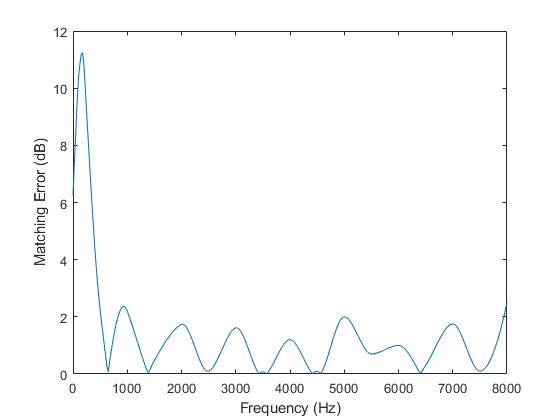
\includegraphics[width=0.6\linewidth]{uniMatErr.PNG}
\caption{Matching Error for Symmetric Filter Bank}
\label{fig:uniMatErr}
\end{figure}  

\section{Symmetric Filter Bank Specifications and Results} 
\label{app:symFreqBands}

\noindent Table \ref{tab:symFreqBand} summarises the frequency bands used to investigate the performance of the symmetric filter bank design. Because the human hearing frequency spectrum begins at $20Hz$, the first sub-band is not symmetric to the last sub-band. However, there is only a $4\%$ difference which is negligible. The transition bandwidth for the first sub-band however, will be $20Hz$. Since only the transition bandwidth of the first sub-band is affected, this affect is also ignored.

% Table generated by Excel2LaTeX from sheet 'Symmetric'
\begin{table}[htbp]
  \centering
  \caption{Symmetric Filter Bank Frequency Bands}
  \begin{adjustbox}{width=0.9\linewidth}
    \begin{tabular}{|r|r|r|r|}
    \hline
    \multicolumn{1}{|l|}{\textbf{Band Number}} & \multicolumn{1}{l|}{\textbf{Lower Passband Frequency $(Hz)$}} & \multicolumn{1}{l|}{\textbf{Upper Passband Frequency $(Hz)$}} & \multicolumn{1}{l|}{\textbf{Bandwidth $(Hz)$}} \\
    \hline
    1     & 20    & 500   & 480 \\
    \hline
    2     & 500   & 1000  & 500 \\
    \hline
    3     & 1000  & 2000  & 1000 \\
    \hline
    4     & 2000  & 4000  & 2000 \\
    \hline
    5     & 4000  & 6000  & 2000 \\
    \hline
    6     & 6000  & 7000  & 1000 \\
    \hline
    7     & 7000  & 7500  & 500 \\
    \hline
    8     & 7500  & 8000  & 500 \\
    \hline
    \end{tabular}%
    \end{adjustbox}
  \label{tab:symFreqBand}%
\end{table}%

\noindent Figure \ref{fig:symMatErr} illustrates the matching error for the full frequency spectrum of the symmetric filter bank.

\begin{figure}[h]
\centering
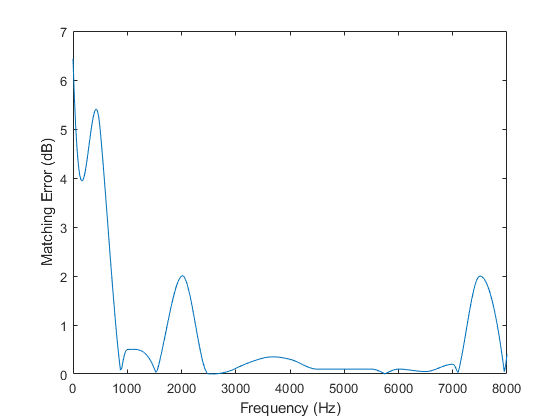
\includegraphics[width=0.6\linewidth]{symMatErr.PNG}
\caption{Matching Error for Symmetric Filter Bank}
\label{fig:symMatErr}
\end{figure}  


\section{Critical-Like Filter Bank Specifications and Results}
\label{app:critFiltFreqBand}

\noindent Within the Bark range, bands 22,23 and 24 fall outside of the $8kHz$ constraint and are therefore, ignored. The remaining 21 bands are divided into 8 sub-bands by grouping together 2 or 3 sub-bands. According to the audiogram used in this design, the greatest hearing loss occurs within the $1kHz$ to $3kHz$ range. Therefore, a greater resolution is required within this frequency range. The frequency bands used in this investigation are therefore given in Table \ref{tab:critFiltFreqBand}.

% Table generated by Excel2LaTeX from sheet 'Bark Scale'
\begin{table}[htbp]
  \centering
  \caption{Frequency Range per Sub-band for Critical-Like Filter Bank}
  \begin{adjustbox}{width=0.9\linewidth}
    \begin{tabular}{|c|r|r|r|r|}
    \hline
    \multicolumn{1}{|l|}{\textbf{Band}} & \multicolumn{1}{l|}{\textbf{Number}} & \multicolumn{1}{l|}{\textbf{Center Frequency (Hz) }} & \multicolumn{1}{l|}{\textbf{Cut-Off Frequency (Hz)}} & \multicolumn{1}{l|}{\textbf{Bandwidth (Hz)}} \\
    \hline
          &       &       & 20    &  \\
    \hline
    \multirow{3}[6]{*}{1} & 1     & 60    & 100   & 80 \\
\cline{2-5}          & 2     & 150   & 200   & 100 \\
\cline{2-5}          & 3     & 250   & 300   & 100 \\
    \hline
    \multirow{3}[6]{*}{2} & 4     & 350   & 400   & 100 \\
\cline{2-5}          & 5     & 450   & 510   & 110 \\
\cline{2-5}          & 6     & 570   & 630   & 120 \\
    \hline
    \multirow{3}[6]{*}{3} & 7     & 700   & 770   & 140 \\
\cline{2-5}          & 8     & 840   & 920   & 150 \\
\cline{2-5}          & 9     & 1000  & 1080  & 160 \\
    \hline
    \multirow{2}[4]{*}{4} & 10    & 1170  & 1270  & 190 \\
\cline{2-5}          & 11    & 1370  & 1480  & 210 \\
    \hline
    \multirow{2}[4]{*}{5} & 12    & 1600  & 1720  & 240 \\
\cline{2-5}          & 13    & 1850  & 2000  & 280 \\
    \hline
    \multirow{2}[4]{*}{6} & 14    & 2150  & 2320  & 320 \\
\cline{2-5}          & 15    & 2500  & 2700  & 380 \\
    \hline
    \multirow{3}[6]{*}{7} & 16    & 2900  & 3150  & 450 \\
\cline{2-5}          & 17    & 3400  & 3700  & 550 \\
\cline{2-5}          & 18    & 4000  & 4400  & 700 \\
    \hline
    \multirow{3}[6]{*}{8} & 19    & 4800  & 5300  & 900 \\
\cline{2-5}          & 20    & 5800  & 6400  & 1100 \\
\cline{2-5}          & 21    & 7000  & 7700  & 1300 \\
    \hline
    \end{tabular}%
    \end{adjustbox}
  \label{tab:critFiltFreqBand}%
\end{table}%

\noindent Figure \ref{fig:critMatErr} provides the matching error of the critical-like filter bank across the full frequency spectrum.

\begin{figure}[h]
\centering
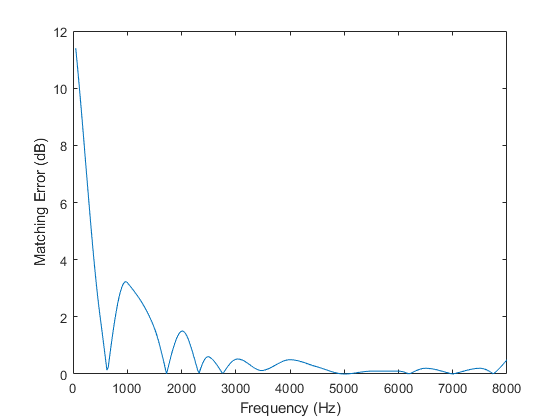
\includegraphics[width=0.6\linewidth]{critMatErr.PNG}
\caption{Matching Error for Critical-Like Filter Bank}
\label{fig:critMatErr}
\end{figure}  




\section{Octave Filter Bank Specifications and Results}
\label{app:octFreqBands}

\noindent Table \ref{tab:octFreqBands} illustrates the frequency bands used in the octave filter bank design. Within the audio range, there exists bands at $16Hz$, $31.25Hz$ and $16kHz$. However, the $16Hz$ and $31.25Hz$ sub-bands are ignored as this design is restricted to using $8$ bands and, $16kHz$ violates the Nyquist sampling criteria.

% Table generated by Excel2LaTeX from sheet 'Octave'
\begin{table}[htbp]
  \centering
  \caption{Octave Filter Bank Frequency Bands}
  \begin{adjustbox}{width=\linewidth}
    \begin{tabular}{|r|r|r|r|}
    \hline
    \multicolumn{1}{|l|}{\textbf{Band}} & \multicolumn{1}{l|}{\textbf{Center Frequency (Hz)}} & \multicolumn{1}{l|}{\textbf{Lower Passband Frequency (Hz)}} & \multicolumn{1}{l|}{\textbf{Upper Passband Frequency (Hz)}} \\
    \hline
    1     & 63    & 45    & 89 \\
    \hline
    2     & 125   & 88    & 177 \\
    \hline
    3     & 250   & 177   & 354 \\
    \hline
    4     & 500   & 354   & 707 \\
    \hline
    5     & 1000  & 707   & 1414 \\
    \hline
    6     & 2000  & 1414  & 2828 \\
    \hline
    7     & 4000  & 2828  & 5657 \\
    \hline
    8     & 8000  & 5657  & 11314 \\
    \hline
    \end{tabular}%
    \end{adjustbox}
  \label{tab:octFreqBands}%
\end{table}%

\noindent Figure \ref{fig:octMatErr} illustrates the matching error of the octave filter bank across the full frequency spectrum.

\begin{figure}[h]
\centering
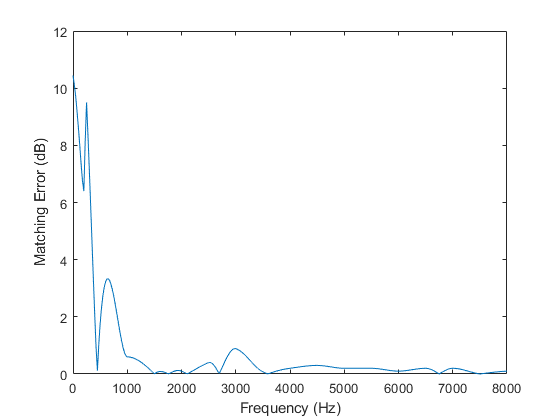
\includegraphics[width=0.6\linewidth]{octMatErr.PNG}
\caption{Matching Error for Octave Filter Bank}
\label{fig:octMatErr}
\end{figure}  


\section{ANSI S1.11 Filter Bank Specifications and Results}
\label{app:ansiSpec}

\noindent Table \ref{tab:ansiFreqSpec} provides the filter specifications for the ANSI S1.11 filter bank. The lower $(f_l)$ and upper $(f_u)$ edge band frequencies are calculated as per equation \ref{eqn:ansiFreqEdge}.

\begin{equation}
\label{eqn:ansiFreqEdge}
\begin{aligned}
f_l &= (G^{-\frac{1}{2b}}) \times f_m \\
f_u &= (G^{\frac{1}{2b}}) \times f_m
\end{aligned}
\end{equation}

\noindent Where $G = 10^{3/10}$ is the octave ratio, $b$ is the bandwidth designator and $f_m$ is the center frequency of the band. Since class $2$ is chosen, the attenuation can range from $-0.5dB$ to $+0.5dB$. An iterative approach is taken to calculating the lower and upper stop band frequencies (i.e. transition bandwidth) to achieve the most accurate frequency response.	

% Table generated by Excel2LaTeX from sheet 'ANSI Oct'
\begin{table}[htbp]
  \centering
  \caption{ANSI S1.11 Filter Bank Frequency Bands}
  \begin{adjustbox}{width=0.9\linewidth}
    \begin{tabular}{|r|r|r|r|r|r|}
    \hline
    \multicolumn{1}{|l|}{\textbf{Sub-band}} & \multicolumn{1}{l|}{\textbf{Lower Stopband Frequency}} & \multicolumn{1}{l|}{\textbf{Lower Passband Frequency}} & \multicolumn{1}{l|}{\textbf{Upper Passband Frequency}} & \multicolumn{1}{l|}{\textbf{Upper Stopband Frequency}} & \multicolumn{1}{l|}{\textbf{Gain}} \\
    \hline
    1     & 1     & 22    & 45    & 145   & -2,42 \\
    \hline
    2     & 30    & 45    & 90    & 190   & -1,27 \\
    \hline
    3     & 60    & 90    & 180   & 280   & 1,26 \\
    \hline
    4     & 80    & 180   & 353   & 535   & 6,69 \\
    \hline
    5     & 153   & 353   & 707   & 907   & 15,62 \\
    \hline
    6     & 507   & 707   & 1403  & 1603  & 23,29 \\
    \hline
    7     & 1203  & 1403  & 2810  & 3010  & 22,07 \\
    \hline
    8     & 2610  & 2810  & 8200  & 8400  & 21,03 \\
    \hline
    \end{tabular}%
    \end{adjustbox}
  \label{tab:ansiFreqSpec}%
\end{table}%

\noindent Figure \ref{fig:ansiOctMatErr} illustrates the matching error for the full frequency spectrum.

\begin{figure}[h]
\centering
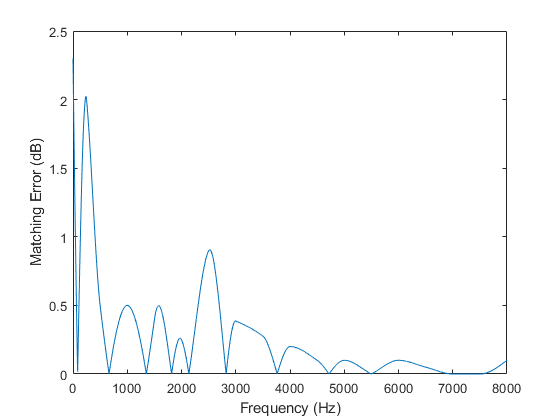
\includegraphics[width=0.6\linewidth]{ansiOctMatErr.PNG}
\caption{Matching Error for ANSI S1.11 Octave Filter Bank}
\label{fig:ansiOctMatErr}
\end{figure} 


\section{Optimised ANSI S1.11 Filter Bank Specifications and Results}
\label{app:ansiOptSpec}

\noindent The frequency specifications were adjusted such that the group delay of the filter bank was less than $10ms$. Table \ref{tab:ansiOptSpec} summarises the specifications for the optimised filter bank.

% Table generated by Excel2LaTeX from sheet 'ANSI Oct'
\begin{table}[htbp]
  \centering
  \caption{Optimised ANSI S1.11 Filter Bank Specifications}
  \begin{adjustbox}{width=0.9\linewidth}
    \begin{tabular}{|r|r|r|r|r|r|}
    \hline
    \multicolumn{1}{|l|}{\textbf{Sub-band}} & \multicolumn{1}{l|}{\textbf{Lower Stopband Frequency $(Hz)$}} & \multicolumn{1}{l|}{\textbf{Lower Passband Frequency $(Hz)$}} & \multicolumn{1}{l|}{\textbf{Upper Passband Frequency $(Hz)$}} & \multicolumn{1}{l|}{\textbf{Upper Stopband Frequency $(Hz)$}} & \multicolumn{1}{l|}{\textbf{Gain $(dB)$}} \\
    \hline
    1     & 10    & 90    & 140   & 240   & 0,47 \\
    \hline
    2     & 60    & 145   & 223   & 323   & 3,16 \\
    \hline
    3     & 123   & 223   & 353   & 535   & 7,60 \\
    \hline
    4     & 153   & 353   & 561   & 761   & 13,68 \\
    \hline
    5     & 361   & 561   & 1100  & 1300  & 21,76 \\
    \hline
    6     & 900   & 1250  & 2220  & 2420  & 22,76 \\
    \hline
    7     & 2020  & 2220  & 4450  & 4650  & 21,23 \\
    \hline
    8     & 4250  & 4450  & 8976  & 9176  & 21,00 \\
    \hline
    \end{tabular}%
    \end{adjustbox}
  \label{tab:ansiOptSpec}%
\end{table}%

\noindent Figure \ref{fig:ansiOptMatErr} illustrates the matching error for the full frequency spectrum.

\begin{figure}[h]
\centering
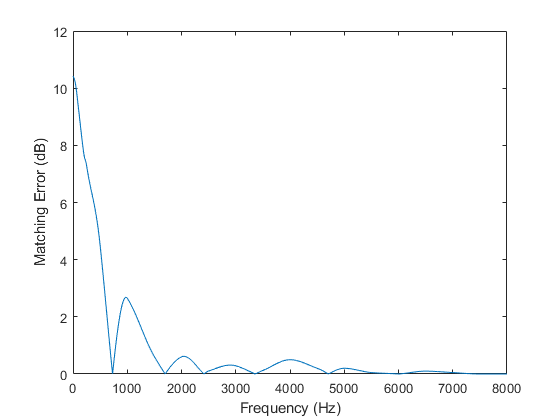
\includegraphics[width=0.6\linewidth]{ansiOptMatErr.PNG}
\caption{Matching Error for Optimised ANSI S1.11 Filter Bank}
\label{fig:ansiOptMatErr}
\end{figure} 

\section{Dynamic Range Compression Parameters}
\label{app:compressPara}

\noindent The Dynamic Range Compression algorithm works by adjusting the output level depending on the input level. These adjustments fit the filter banks output into a suitable loudness range. The specifics of the parameters used in the dynamic range compression algorithm are discussed below.

\begin{itemize}
	\item Compression Threshold: The compression threshold is the point where the compression algorithm begins to compress the loudness levels. This is also referred to as the threshold knee point and defined as the point where the output level is $2dB$ lower than the uncompressed output level.
	\item Compression Ratio: This parameter (shown in equation \ref{eqn:cr}) defines how much the input signal will be compressed, once above the compression threshold. 
	\begin{equation}
	\label{eqn:cr}
		CR = \frac{\Delta input}{\Delta output}
	\end{equation}
	\noindent Below the compression threshold, the compression ratio is $1$.
	\item Attack Time: The attack time is the delay from when the input signal surpasses the compression threshold, to when the compression takes affect.
	\item Release Time: Release time is measured as the time between when the input loudness level drops below the compression threshold, to when the compression deactivates.
\end{itemize}

\section{Dynamic Range Compression Calculations}
\label{app:compressCalc}

\noindent Reference \cite{compCalc} provides the calculations presented in this section. The input signal is sampled $(x[n])$ and converted to decibels ($x_{dB}[n] = 20\times log_{10}|x[n]|$). This design utilises a hard knee and hence, the static characteristics are calculated as shown in equation \ref{eqn:staticCharac}.

\begin{equation}
\label{eqn:staticCharac}
x_{sc}(x_{dB}) = 
\begin{cases} 
      x_{dB} & x_{dB} < T \\
     T + \frac{x_{dB} - T}{R} & x_{dB} \geq T
   \end{cases}
\end{equation}

\noindent Where $T$ is the compression threshold and $R$ is the compression ratio. The gain is then calculated by taking the difference between the static characteristics and the input signal $(g_c[n] = x_{sc}[n] - x_{dB}[n])$. The attack and release parameters are then applied to the gain as shown in equation \ref{eqn:gainSmooth}.

\begin{equation}
\label{eqn:gainSmooth}
g_s[n] = 
\begin{cases} 
      \alpha_A g_s[n-1] + (1-\alpha_A)g_c[n] & g_c[n] \leq g_s[n-1] \\
     \alpha_R g_s[n-1] + (1-\alpha_R)g_c[n] & g_c[n] > g_s[n-1]
   \end{cases}
\end{equation}

\noindent Where $g_s$ is the smoothed gain and $\alpha_A$ and $\alpha_R$ are the attack and release time coefficients calculated as shown in equation \ref{eqn:attackCoeff} and \ref{eqn:releaseCoeff} respectively.
%
\begin{equation}
\label{eqn:attackCoeff}
\alpha_A = e^{\frac{-log(9)}{F_s\times T_A}}
\end{equation}
%
\begin{equation}
\label{eqn:releaseCoeff}
\alpha_R = e^{\frac{-log(9)}{F_s\times T_R}}
\end{equation}
%
\noindent Where $T_A$ and $T_R$ are the attack and release times respectively. The make-up gain $M$, is calculated such that a $0dB$, stead state input will give a $0dB$ steady state output. Equation \ref{eqn:makeUpGain} describes how this value is obtained.
%
\begin{equation}
\label{eqn:makeUpGain}
M = T - (T/R)
\end{equation}
%
\noindent The make-up gain is then applied to the smoothed gain $(g_m = g_s[n] + M)$. The value $g_m$ has units of $(dB)$ and therefore, the equivalent linear value $(g_{lin})$, must be calculated. This is achieved using equation \ref{eqn:glin}.

\begin{equation}
\label{eqn:glin}
g_{lin} = 10^{\frac{g_m[n]}{20}}
\end{equation}

\noindent Finally, the output $(y)$ is calculated as shown in equation \ref{eqn:compressOutput}.

\begin{equation}
\label{eqn:compressOutput}
y[n] = x[n] \times g_{lin}[n]
\end{equation}


\section{Testing and Results}
\label{app:test}

\noindent This appendix contacts the various experimentation set-ups and results used to evaluate the success of the design.

\subsection{Matching Error Testing and Results}
\label{app:testMatErr}

\noindent To investigate the conversational performance of the system, the experimentation set-up, illustrated in Figure \ref{fig:matErrTest} is used.

\begin{figure}[h]
\centering
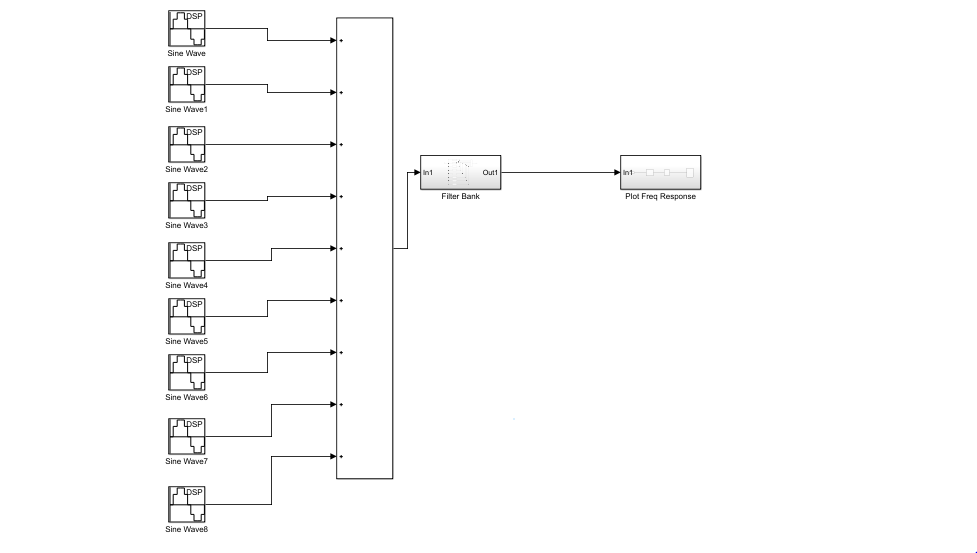
\includegraphics[width=0.6\linewidth]{matErrTest.PNG}
\caption{Dynamic Range Compressor Static Characteristics}
\label{fig:matErrTest}
\end{figure}

\FloatBarrier
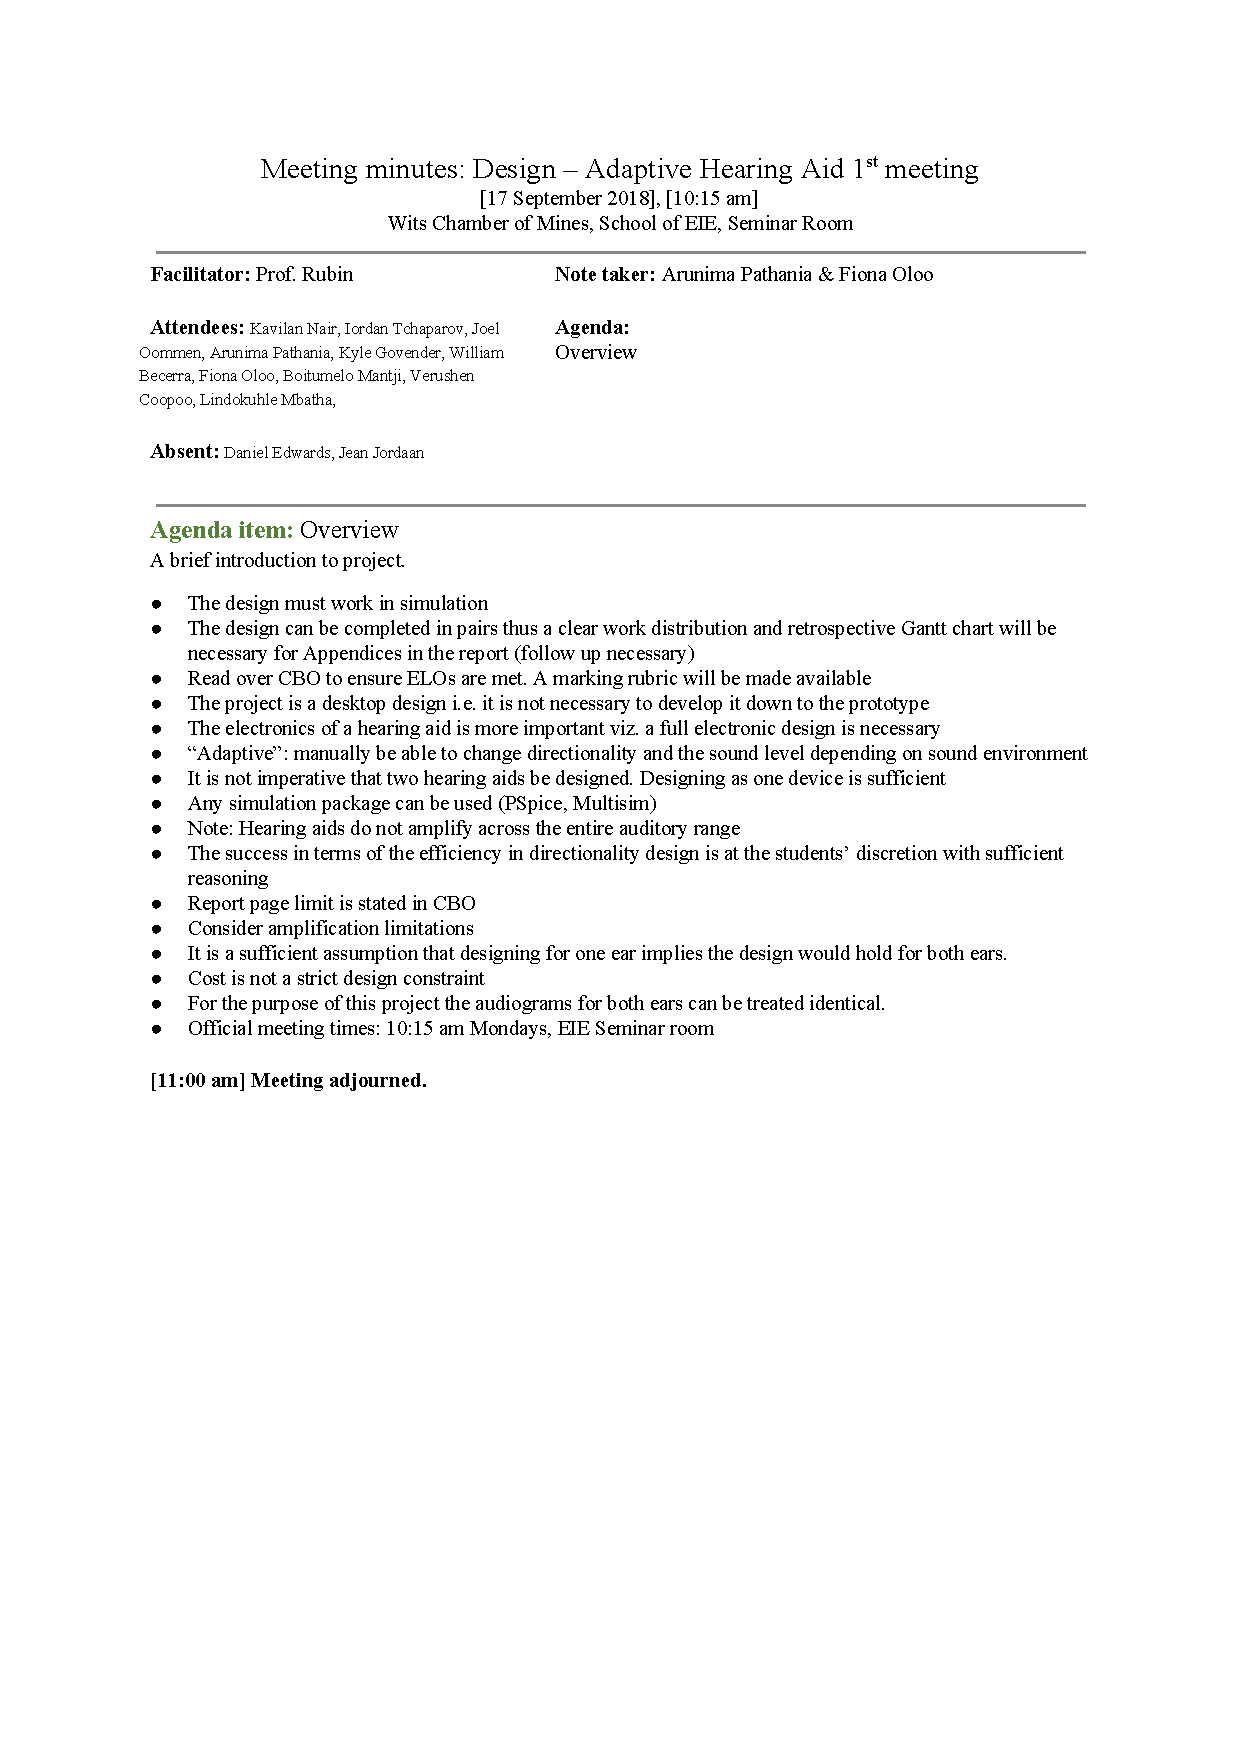
\includepdf[pages=-, picturecommand*={%
	\put(45,750){%change this put command to fit your document
		\parbox{\textwidth}{\section{Meeting Minutes}\label{app:plan}}
	}}]{meetingMin.pdf}


\end{appendices}
\end{document}
